\chapter{Discussion}\label{chapter:discussion}
% TODO: Needs citations!

\section{Introduction}
In this chapter, I contextualise the results of the study through the lens of the three research questions outlined in Chapter~\ref{chapter:introduction} and the broader research field within which they are situated. The empirical findings reveal several interesting patterns that suggest areas for further investigation in collaborative AR design, while confirming certain technical challenges identified in the literature review.

\section{RQ1: Classification of human-human AR collaboration in industrial applications}
As explained in Chapter~\ref{chapter:artifact-implementation}, I positioned the design of the user study within the 'Collaborative Creative Workflows' archetype (outlined in Chapter~\ref{chapter:literature}), which is characterised by many-to-one information flow, direct manipulation, co-creation, and a focus on the creative process. The results of the study confirm that the bridge task aligns well with this archetype, featuring many-to-one information flow through a central shared bridge model and direct manipulation via gestural control, focused on co-creation.

However, due to its shared-space human-human nature, the bridge task also mirrors traditional, shared-space industrial assembly tasks, which introduces additional constraints and characteristics not fully captured in the existing literature's focus on creative workflows more generally\cite{vidalBalea2020creating}. The empirical findings reveal several distinguishing features:

\begin{itemize}
    \item \textbf{Spatial deixis patterns:} Consistent spatial deixis (approximately 6.5\% of verbal communication across variants), a characteristic of manual assembly that has been observed in human-robot collaboration \cite{sauppe2014robot}. This proportion remained remarkably stable across all verbal communication variants despite differences in session duration and total word counts.
    \item \textbf{Movement synchronisation:} Strong correlation between participants' movement patterns ($\rho = 0.737, p < 0.001$), mirroring the joint-action adaptation observed in non-AR collaborative assembly tasks \cite{sebanz2006joint}. This contrasts with remote collaboration, where movement data must be explicitly transmitted or may be omitted entirely.
    \item \textbf{Template development and reuse patterns:} Systematic development of reusable construction procedures that mirror standard work practices \cite{kamrani2006methodology}, enabling cross-variant learning and skill transfer. This led to quality-speed independence, where bridge structural performance remained consistent despite 3-fold variation in completion times.
    \item \textbf{Resource optimisation behaviours:} Participants consistently chose cost-efficient, ground-level solutions over aesthetically-driven designs, demonstrating industrial efficiency mindset over creative expression.
\end{itemize}

\subsection{Implications for Industrial Collaboration Taxonomy}
The empirical findings listed above reveal that the existing Collaborative Creative Workflows archetype, while appropriate for capturing the general characteristics of the bridge task, requires refinement to more precisely represent the unique dynamics observed in shared-space AR manual assembly contexts. The distinct characteristics suggest value in developing more specialised classification approaches that better capture these specific interaction patterns.

The distinguishing features identified collectively point toward a specialised variant that could be termed \textbf{Co-located Industrial Assembly}. This sub-archetype would encompass collaborative tasks characterised by shared physical workspace, structured quantitative quality requirements, resource optimisation pressures, and the potential for standardised procedures. It differs meaningfully from other applications within Collaborative Creative Workflows, such as remote design review or artistic co-creation, in several key dimensions: (1) the emphasis on efficiency and resource optimisation over aesthetic exploration, (2) the beneficial effects of communication constraints rather than enhanced communication capabilities, (3) the central role of movement synchronisation and spatial coordination, and (4) the systematic development of reusable procedural templates.

\subsection{Template Development as Industrial Learning Pattern}
One of the most notable behavioural patterns that emerged was participants' systematic development of reusable construction templates across task variants. This template development process closely mirrors standard work practices in industrial manufacturing, where workers iteratively refine procedures to achieve optimal efficiency and quality outcomes \cite{kamrani2006methodology}.

The observed template development directly parallels how skilled industrial workers develop efficient methods through repetition, gradually optimising their approach based on experience and feedback. This learning pattern explains the unexpected success of the Silent condition, where cross-variant adaptation enabled effective non-verbal coordination despite communication constraints. The ability to leverage established spatial patterns and construction sequences demonstrates how collaborative knowledge becomes embodied through practice.

Figure~\ref{fig:bridge_contrast_traditional_vs_optimized} illustrates the template development process via two examples of dyads. The first dyad (top row) maintains traditional engineering principles, while the second dyad (bottom row) optimises for resource efficiency. Both approaches represent systematic template development and reuse across task variants.

\begin{figure}[H]
\centering
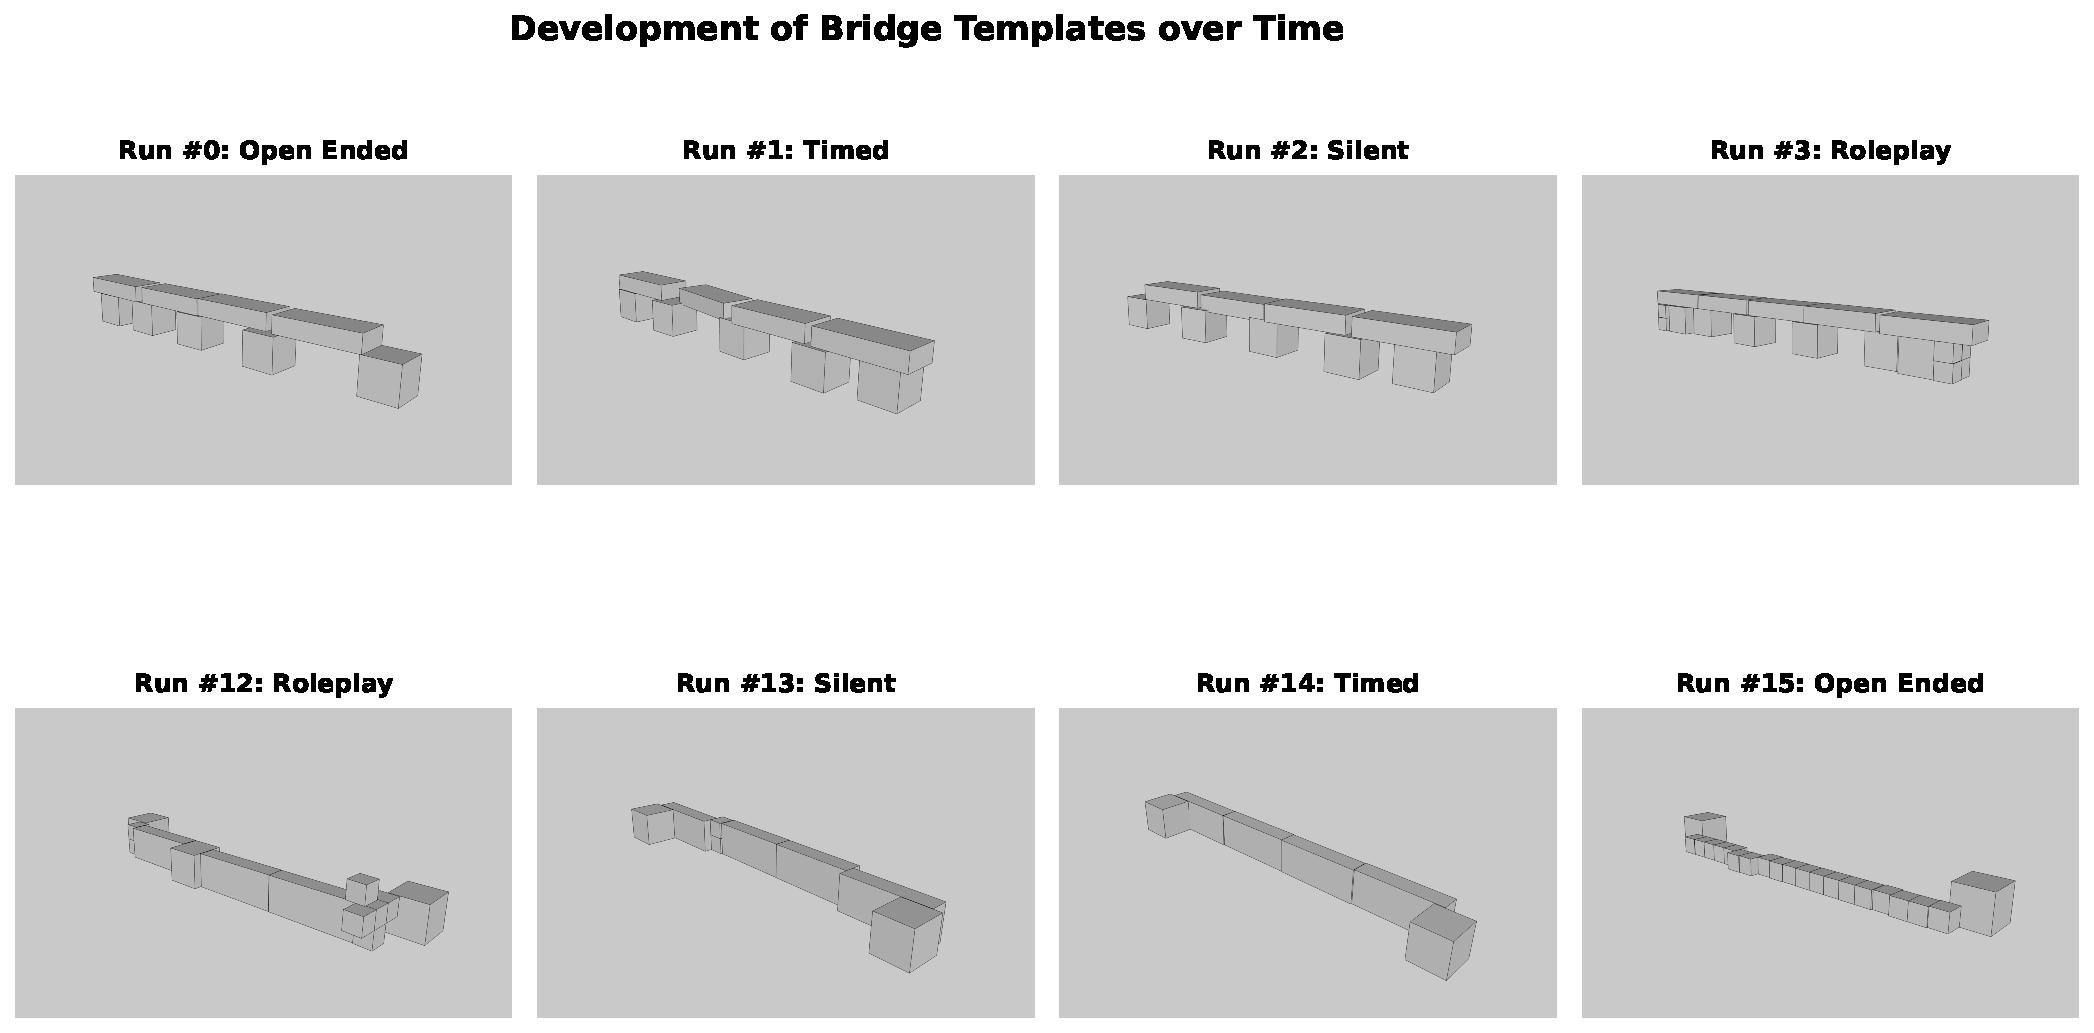
\includegraphics[width=\textwidth]{assets/06/bridge_contrast_traditional_vs_optimized.pdf}
\caption{Development of bridge construction templates across task variants. The top row shows traditional engineering approaches maintaining vertical structural elements, while the bottom row demonstrates resource-optimised ground-level solutions. Both approaches represent systematic template development and reuse across all four experimental conditions.}
\label{fig:bridge_contrast_traditional_vs_optimized}
\end{figure}

This finding suggests that collaborative AR systems could benefit from explicitly supporting pattern recognition and template reuse capabilities, rather than treating each interaction as independent. The learning transfer observed between variants indicates that well-designed industrial AR applications should incorporate mechanisms for capturing, storing, and retrieving successful collaborative patterns.

The industrial parallel is particularly relevant for training systems and knowledge transfer applications. Just as experienced factory workers develop tacit knowledge about efficient assembly sequences, collaborative AR users demonstrate rapid development of spatial and temporal coordination patterns that can be transferred across similar tasks.

\subsection{Synthesis: Towards Refined Industrial AR Collaboration Models}
The empirical analysis of RQ1 suggests that while existing collaboration archetypes provide a useful foundation, the specific characteristics of shared-space industrial AR collaboration may warrant more nuanced classification approaches. The identification of spatial deixis patterns, movement synchronisation, template development, and resource optimisation behaviours collectively suggest a potentially distinct "Co-located Industrial Assembly" sub-archetype that might capture the unique dynamics observed in manufacturing contexts. The systematic template development and cross-variant learning patterns suggest that collaborative AR systems might benefit from explicitly supporting knowledge transfer mechanisms rather than treating each interaction independently, aligning with established industrial learning principles while extending them into augmented reality environments. However, these observations require validation in larger studies before firm conclusions can be drawn.

\section{RQ2: Technical Architecture Challenges and Solutions}
In Chapter~\ref{chapter:literature}, I identified four main challenges associated with the technical architecture of collaborative AR systems: hardware constraints, tracking accuracy, network communication, and system performance. During implementation and evaluation of the artifact, I confirmed that these four challenges represent the primary technical barriers encountered in developing shared-space collaborative AR systems for industrial applications.

\subsection{Hardware Constraints and Ergonomic Limitations}
While user feedback on the HoloLens 2 was generally positive, hardware constraints emerged as significant barriers to extended use. The headset required charging between task variants, and overheating during one session necessitated air conditioning for all subsequent sessions. These findings align with the literature's identification of ergonomic constraints as persistent challenges \cite{cogurcu2023comparative, yang2023usability}.

The System Usability Scale progression (67.5 → 72.5, p = 0.015) demonstrated that users adapt to hardware limitations over time, with learning effects strongest for participants with limited AR/VR experience (+9.6 points improvement). However, the need for such adaptation suggests that hardware ergonomics remain a deployment barrier for extended industrial applications.

\subsection{Spatial Tracking and Registration Accuracy}
Spatial tracking accuracy proved both critical and challenging in the multi-user shared-space scenario. Despite implementing a robust two-stage calibration system with marker-based tracking, tracking drift occurred in 2 of 32 sessions during extended use (both during Roleplay sessions approaching 30 minutes). The geometric median and Karcher mean approach provided sub-millimetre precision during calibration, with theoretical alignment guarantees of $\leq45 mm$ translation and $\leq1.03°$ rotation error.

However, the calibration process itself presented usability challenges. Manual calibration procedures were necessary before each task variant to counter drift in extended sessions, which is viable in controlled environments but unlikely to be acceptable in real-world industrial settings. As one participant noted: "Calibration sucked, but everything else was fine" (Participant 7), while another commented: "Frustrated at the beginning because the thing wasn't calibrating, but once I got the hang of it... it was very, very easy" (Participant 4).

The literature's emphasis on marker-based tracking systems for collaborative scenarios \cite{martins2024multiUser} proved correct, as the headset-internal spatial anchors used by most studies would likely have introduced more frequent misalignment issues.

\subsection{Network Communication and Latency Management}
The networking architecture achieved its design targets, with average round-trip latency of 25.72 $\pm$ 8.85 ms on localhost and theoretical total latency of 35.72 $\pm$ 8.85 ms including wireless networking—well within the 50 ms target for real-time interactive systems \cite{sonkoly2024edge}. Bandwidth requirements remained minimal (1.26 $\pm$ 2.51 kbps outbound), providing substantial headroom for scaling to multiple concurrent users.

Despite this technical success, network communication issues remained perceptible to participants. Minor lag spikes, while not disruptive to task completion, created awareness of system limitations: "What I didn't like was when we saw different realities, when I spawned the parts and then they didn't show up or they showed up as like 20 parts a few seconds later" (Participant 1).

Interestingly, participants demonstrated resilience to these technical difficulties, developing adaptive strategies rather than failing to complete tasks: "For the person for who the system works best, like took the lead in building and like the other just checked what they were doing" (Participant 1). This adaptation pattern suggests that robust collaboration frameworks can overcome technical imperfections through natural human problem-solving capabilities.

\subsection{System Performance and Computational Constraints}
The performance constraints identified in the literature review \cite{reis2021caseStudy, schmidt2022augmentedReality} proved accurate for the HoloLens 2 platform. Complex virtual content and physics simulations required careful optimisation to maintain acceptable frame rates. While primarily a UX design decision, the simplified block layout used in the study exemplifies the type of system-level optimisation needed to achieve stable collaborative interactions within hardware limitations.

Grid-snapping for placement stability addressed precision challenges while maintaining construction efficiency, though some participants noted trade-offs in fine-grained placement control. This compromise between precision and stability reflects broader tensions in collaborative AR system design between technical capability and user expectations \cite{neumann1998cognitive}.

\subsection{Implications for Industrial Deployment}
The technical evaluation suggests that current AR hardware may support effective collaborative applications, but with important constraints. The combination of marker-based tracking, optimised networking, and adaptive physics provides a foundation for shared-space collaboration, while hardware limitations and calibration requirements suggest that deployment strategies should accommodate these constraints rather than attempting to eliminate them entirely.

For industrial applications, the findings suggest a potentially viable phased deployment approach: starting with controlled environments that can accommodate fragile hardware and calibration procedures, using marker-based tracking for reliability, implementing optimised networking protocols, and designing tasks that can benefit from or at least cope with current hardware limitations.

\subsection{Synthesis: Technical Feasibility Within Defined Constraints}
The technical architecture evaluation suggests that collaborative AR systems may effectively support industrial applications, while highlighting the importance of working within current technological constraints rather than attempting to overcome them entirely. The implementation of shared-space collaboration through marker-based tracking, optimised networking, and adaptive system design demonstrates preliminary technical viability, though hardware limitations and calibration requirements suggest that deployment strategies should accommodate these realities. The adaptive behaviours observed when participants encountered technical difficulties suggest that robust collaboration frameworks might maintain effectiveness despite technical imperfections.

\section{RQ3: System Influence on Collaboration Dynamics}
The empirical findings reveal several unexpected patterns regarding how AR system design influences collaboration dynamics, suggesting that some common assumptions about communication, time pressure, and performance relationships may warrant further investigation.

\subsection{Communication Constraints as Performance Enhancers}
One of the most striking findings was that communication constraints appeared to enhance rather than hinder collaborative performance. This unexpected result suggests that well-designed constraints might focus collaborative effort more effectively than open-ended conditions, though this finding requires validation in larger studies.

This preliminary finding raises questions about the assumption that enhanced communication capabilities inherently improve collaboration. Instead, the results suggest that communication efficiency may matter more than communication volume. The Silent condition's success reveals how participants leveraged embodied knowledge and spatial coordination patterns developed through prior experience, achieving smooth execution without verbal negotiation overhead.

The consistency of spatial coordination language patterns across different task variants suggests that certain communication elements represent fundamental collaborative requirements, independent of external constraints. This points toward a more nuanced understanding of how communication supports collaboration, where focused interaction may be more valuable than unrestricted discussion.

\subsection{Time Pressure and Quality Independence}
The Timed condition demonstrated that external time pressure can drive efficiency improvements without compromising structural quality. The observed quality-speed independence across all task variants suggests that collaborative AR systems can accommodate varying time constraints without sacrificing output quality, provided that participants have sufficient experience with the task and system.

This finding may have implications for industrial applications, where both efficiency and quality requirements must be satisfied simultaneously. It suggests that time pressure, when applied appropriately, might enhance focus and eliminate inefficient coordination behaviors without degrading collaborative outcomes. This raises questions about the assumption that rushed work necessarily compromises quality in collaborative contexts, though further validation is needed.

\subsection{Movement Synchronisation and Coordination Patterns}
The strong correlation between partners' movement per minute ($\rho = 0.737, p < 0.001$) varied systematically across task variants, ranging from near-perfect matching under time pressure ($\rho = 0.939$) to weaker matching in silent conditions ($\rho = 0.351$). This variation suggests that different collaboration constraints influence whether partners engage with similar activity levels, revealing how system design affects fundamental coordination mechanisms.

Individual dyads maintained consistent activity level patterns across variants, indicating stable partnership characteristics that persist despite changing task demands. This finding suggests that collaborative AR systems should accommodate different partnership styles rather than imposing uniform interaction patterns.

\subsection{Task Ambiguity as Collaborative Driver}
The study revealed fundamental disagreements about what constitutes a "bridge," representing a microcosm of broader tensions in industrial work environments. Rather than representing a design flaw, this controversy functioned as productive ambiguity that channelled different collaborative approaches and forced conceptual negotiation.

This reflects fundamental tensions present in industrial work: the conflict between technical idealism and operational efficiency. Most dyads demonstrated evolution toward pragmatic compromise as they experienced multiple task variants, mirroring how production targets influence decision-making in manufacturing environments.

This finding suggests that well-designed ambiguity can enhance rather than hinder collaborative effectiveness by forcing teams to explicitly negotiate their approach and establish shared frameworks. Task definitions often evolve under operational constraints, and successful collaborative systems must accommodate this evolution rather than enforcing rigid interpretations.

\subsection{Individual Differences and Adaptation Patterns}
While personality traits showed weak correlations with performance outcomes, qualitative analysis revealed that individual differences influenced collaboration approaches in meaningful ways. Openness to experience showed the strongest relationship with task completion speed ($\rho = -0.409$), suggesting that individuals more receptive to new experiences may adapt more quickly to collaborative AR construction tasks.

AR/VR experience demonstrated complex non-linear relationships with both performance and learning outcomes. Participants with extensive experience achieved the fastest completion times (6.41 $\pm$ 2.15 minutes), while those with limited experience showed the strongest usability improvements (+9.6 SUS points), indicating that collaborative AR systems can accommodate users with varying technical backgrounds through adaptive learning processes.

\subsection{Implications for Collaborative AR Design}
These preliminary findings suggest several potential design principles for collaborative AR systems in industrial contexts that warrant further investigation:

\textbf{Consider constraint-driven efficiency:} Well-designed constraints (time pressure, communication limits) might focus collaborative effort more effectively than open-ended conditions, though this challenges the assumption that more communication capabilities automatically improve collaboration and requires validation in larger studies.

\textbf{Consider supporting template development and reuse:} The systematic development of reusable construction patterns appeared crucial for collaboration success, suggesting that systems might benefit from enabling pattern recognition and knowledge transfer rather than treating each interaction independently.

\textbf{Accommodate diverse collaboration approaches:} Rather than imposing uniform interaction patterns, systems might benefit from supporting the different working styles and priorities that emerge naturally in industrial contexts.

\textbf{Consider productive ambiguity:} Task definitions that require negotiation might enhance collaboration depth by forcing teams to establish shared frameworks and priorities, mirroring real industrial work dynamics.

These exploratory results suggest that collaborative AR systems may be able to effectively support industrial assembly tasks while revealing complex relationships between system design, collaboration constraints, and performance outcomes that warrant further investigation in larger-scale studies.
